\subsubsection{哈希表}

\begin{minted}{cpp}
#include<ext/pb_ds/assoc_container.hpp>
#include<ext/pb_ds/hash_policy.hpp>
using namespace __gnu_pbds;

cc_hash_table<string, int> mp1; // 拉链法
gp_hash_table<string, int> mp2; // 查探法(快一些)
\end{minted}

\subsubsection{堆}

默认也是大根堆, 和\mintinline{cpp}{std::priority_queue}保持一致.

\begin{minted}{cpp}
#include<ext/pb_ds/priority_queue.hpp>
using namespace __gnu_pbds;

__gnu_pbds::priority_queue<int> q;
__gnu_pbds::priority_queue<int, greater<int>, pairing_heap_tag> pq;
\end{minted}

效率参考:

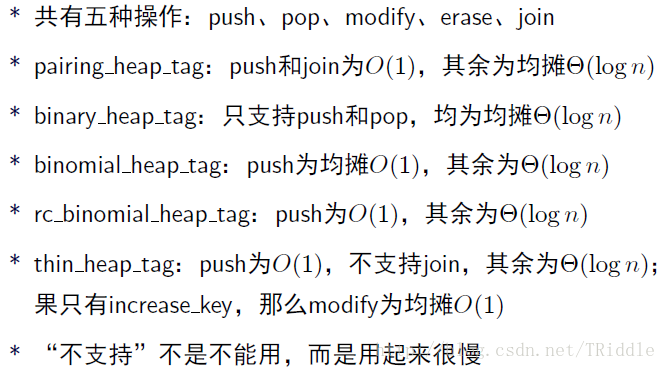
\includegraphics[scale = 0.385]{../src/misc/pbds_heap.png}

常用操作:

\begin{itemize}

	\item \mintinline{cpp}{push()}: 向堆中压入一个元素, 返回迭代器
	\item \mintinline{cpp}{pop()}: 将堆顶元素弹出
	\item \mintinline{cpp}{top()}: 返回堆顶元素
	\item \mintinline{cpp}{size()}: 返回元素个数
	\item \mintinline{cpp}{empty()}: 返回是否非空
	\item \mintinline{cpp}{modify(point_iterator, const key)}: 把迭代器位置的 \mintinline{cpp}{key} 修改为传入的 \mintinline{cpp}{key}
	\item \mintinline{cpp}{erase(point_iterator)}: 把迭代器位置的键值从堆中删除
	\item \mintinline{cpp}{join(__gnu_pbds::priority_queue &other)}: 把 \mintinline{cpp}{other} 合并到 \mintinline{cpp}{*this}, 并把 \mintinline{cpp}{other} 清空
\end{itemize}

\subsubsection{平衡树}

\begin{minted}{cpp}
#include <ext/pb_ds/tree_policy.hpp>
#include <ext/pb_ds/assoc_container.hpp>
using namespace __gnu_pbds;

tree<int, null_type, less<int>, rb_tree_tag, tree_order_statistics_node_update> t;

// rb_tree_tag 红黑树(还有splay_tree_tag和ov_tree_tag, 后者不知道是什么)
\end{minted}

注意第五个参数要填\mintinline{cpp}{tree_order_statistics_node_update}才能使用排名操作.

\begin{itemize}
	\item \mintinline{cpp}{insert(x)}: 向树中插入一个元素x, 返回\mintinline{cpp}{pair<point_iterator, bool>}
	\item \mintinline{cpp}{erase(x)}: 从树中删除一个元素/迭代器x, 返回一个 \mintinline{cpp}{bool} 表明是否删除成功
	\item \mintinline{cpp}{order_of_key(x)}: 返回x的排名, 0-based
	\item \mintinline{cpp}{find_by_order(x)}: 返回排名(0-based)所对应元素的迭代器
	\item \mintinline{cpp}{lower_bound(x) / upper_bound(x)}: 返回第一个$\ge$或者>x的元素的迭代器
	\item \mintinline{cpp}{join(x)}: 将x树并入当前树, 前提是两棵树的类型一样, 并且二者值域不能重叠, x树会被删除
	\item \mintinline{cpp}{split(x,b)}: 分裂成两部分, 小于等于x的属于当前树, 其余的属于b树
	\item \mintinline{cpp}{empty()}: 返回是否为空
	\item \mintinline{cpp}{size()}: 返回大小
\end{itemize}

(注意平衡树不支持多重值, 如果需要多重值, 可以再开一个\mintinline{cpp}{unordered_map}来记录值出现的次数, 将\mintinline{cpp}{x<<32}后加上出现的次数后插入. 注意此时应该为long long类型.)